\chapter{関連研究}
\label{chap:relatedResearch}

本章では関連研究を紹介し、それらの特徴や本研究との関連性について示す。

\newpage


\section{主要な研究領域}
本研究ではNFCのタッチインタラクション及びwikiベースなARナビゲーションが有用であることを検討した。
本研究に関連する先行研究は大きく以下のように分類できる
\begin{itemize}
  \item ARをナビゲーションに利用する研究
  \item ユーザの位置測位及びコンテキスト情報の取得に関する研究
  \item NFCを用いて情報を取得し、ナビゲーションに応用する研究
  \item AR情報の整理・関連情報推薦にハイパーリンクを利用する研究
\end{itemize}
それぞれについて関連性の高いものを紹介した上で本研究との関連性を示す。

\section{ARをナビゲーションに利用する研究}
ARを地理情報のナビゲーションとして利用する代表的な研究及びシステムを紹介する。

\subsection{A Touring Machine}
Feinerらが開発したA Touring Machine\cite{629922}(図\ref{fig:a_touring_machine})はヘッドマウント・ディスプレイとスタライスで操作可能な2Dディスプレイで大学のキャンパスの情報を表示するアプリケーションである。
ARを利用した地理情報ナビゲーションの初期研究として挙げられる。
GPSによる位置情報と磁気センサによる向きの情報からユーザーの位置と向きを推定し、ヘッドマウント・ディスプレイに大学の情報が表示される。
また手持ちのスタライスで操作可能な2Dディスプレイが専用のHTTPサーバにつながっており、表示したい情報のリンクに触れるなどの操作することでヘッドマウント・ディスプレイでの表示情報が変化するようになっている。
一方でGPSと磁気センサによる位置推定には精度の面で課題があり、当時の技術ではヘッドマウント・ディスプレイとコンピュータを小型化することが難しかったため常用するには難しいものであった。

\begin{figure}[h]
  \centering 
  
\includegraphics[width=150mm]{images/wip.jpg}
  \caption{A Touring Machine} \label{fig:a_touring_machine}
\end{figure}


\subsection{KARMA}
同じくFeinerらがKnowledge-based augmented reality\cite{10.1145/159544.159587}で提案したKARMA(図\ref{fig:karma})はレーザープリンターのメンテナンスをARで説明するプロトタイプシステムである。
ヘッドマウント・ディスプレイによってレーザープリンターの内部機構に関する情報を提示しメンテナンスを助けるものであった。
位置測位は超音波センサを利用しておりこれらのセンサをすべての対象に取り付ける必要があるという難点があった。

\begin{figure}[h]
  \centering
  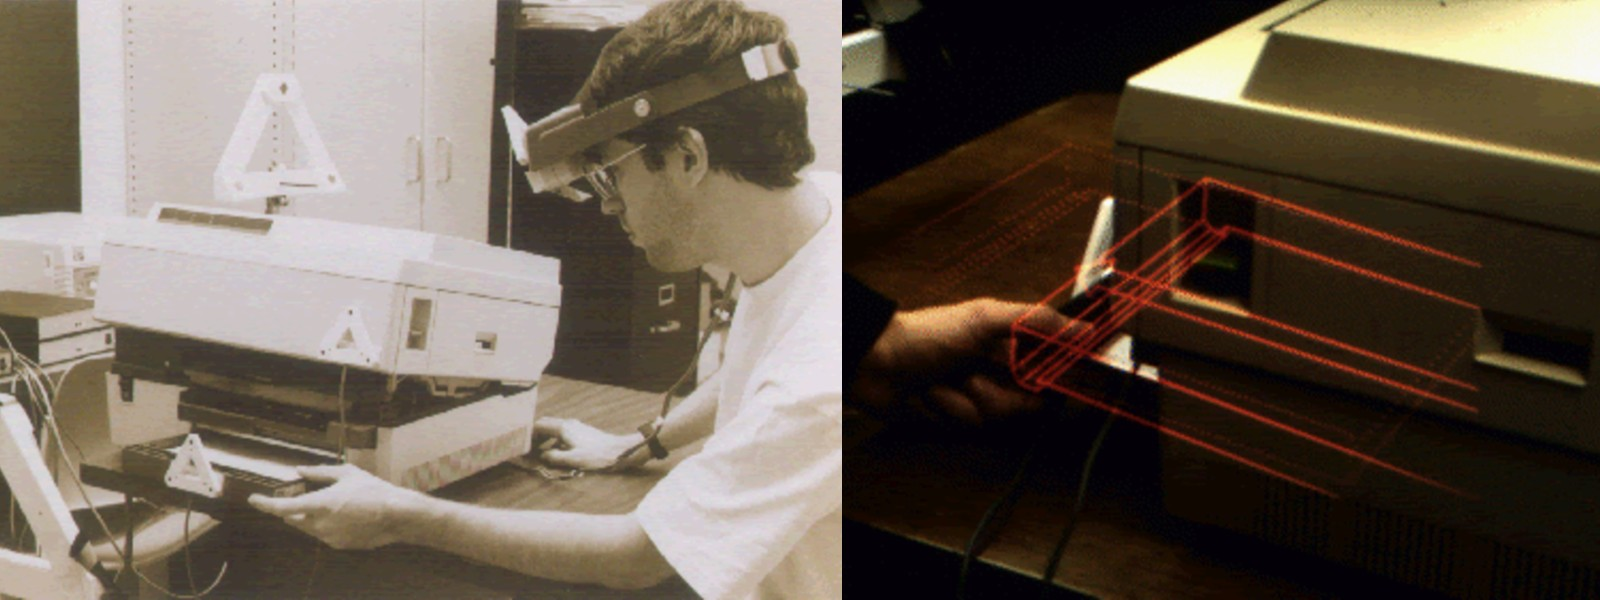
\includegraphics[width=150mm]{images/karma.jpg}
  \caption{KARMA} \label{fig:karma}
\end{figure}


\subsection{MARS}
HöllererらによるMARS\cite{MARS}は上記の「A Touring Machine」及び「KARMA」の方式を組み合わせ、屋内と屋外の両方でヘッドマウントディスプレイによるナビゲーションを可能にするプロトタイプである。


% \begin{figure}[h]
%   \centering
%   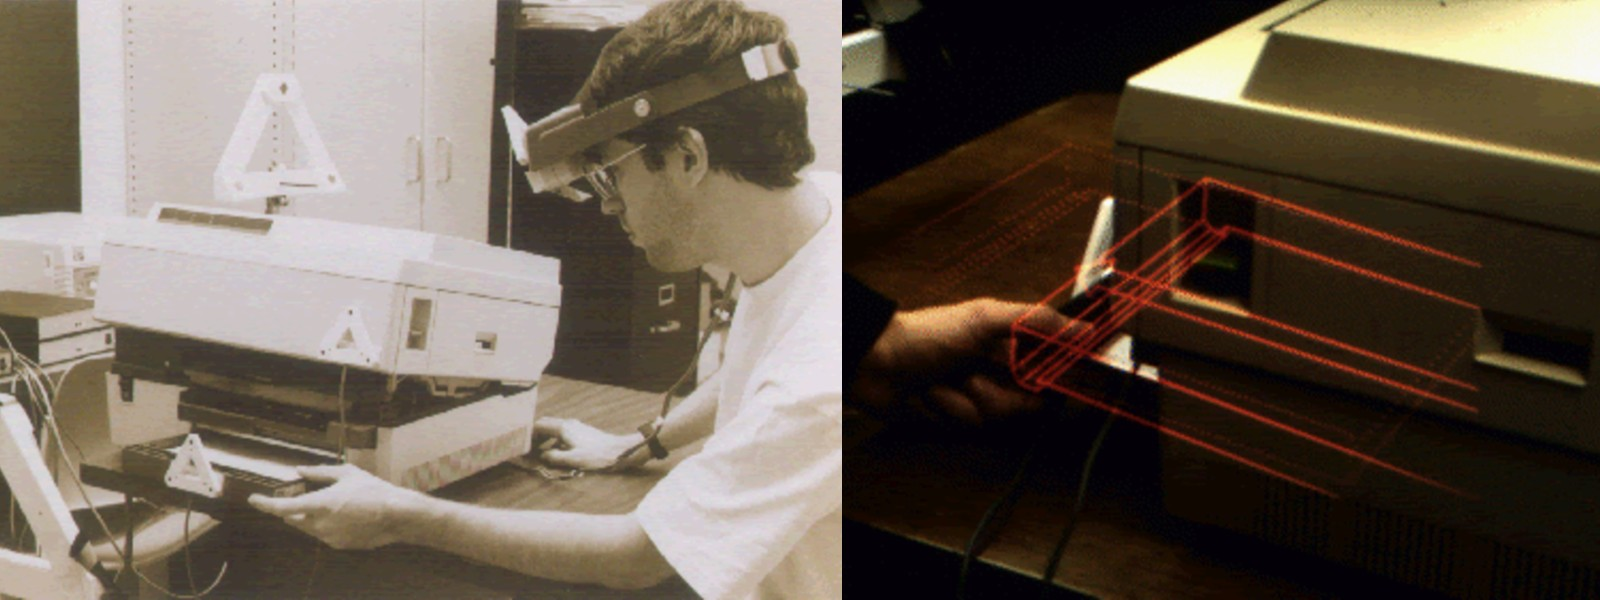
\includegraphics[width=150mm]{images/karma.jpg}
%   \caption{KARMA} \label{fig:karma}
% \end{figure}

\subsection{NaviCam}
暦本らによるNaviCam\cite{10.1145/215585.215639}はマーカーをカメラで認識し、マーカー応じてその場に即した説明を手持ちの2Dディスプレイやヘッドマウントディスプレイに提示するシステムである。
現在主流になっているマーカーベースのARの初期研究であり、青と赤の線で構成されたカラーコードと呼ばれるバーコードを認識することで状況と対象物の位置を把握し、情報を提示している。


\begin{figure}[h]
  \centering
  
\includegraphics[width=150mm]{images/wip.jpg}
  \caption{NaviCam} \label{fig:NaviCam}
\end{figure}




\subsection{Feature-Based Indoor Navigation Using Augmented Reality}
KasprzakらはFeature-Based Indoor Navigation Using Augmented Reality\cite{6597797}で室内での利用を想定したモバイル端末のARナビゲーションのプロトタイプを作成し評価している。
このプロトタイプは画像として登録された特徴的なアイコンなどを元に画像認識から位置情報と向きを推定し、ユーザーの目的地を矢印で表示するものである。
またこのプロトタイプを利用し、実際に建物内での案内に利用するテストを行っている。
その結果2Dの地図と比べて目的地までの到達時間が短縮され、被験者が立ち止まったり間違えた方向に進む回数も減少したと報告している。
室内での利用を視野に入れている点はGPSなどを利用するシステムと違い、本研究に近いが登録した画像による位置推定には以下のような課題もある。
\begin{itemize}
  \item 特徴的なロゴやアイコンの無いところでは登録できる画像がなく精度が保証できない
  \item 各場所で個別に画像の登録が必要
  \item 距離や明るさなどによっては認識できない可能性がある
\end{itemize}
またこのプロトタイプシステムでは事前に選択した目的地に正確に早く到着することに主眼を置いており、本システムのようにハイパーリンクによる関連情報から周辺譲歩を探索する用途を考えていない点も本研究との違いである。

\subsection{Wikitude}
Wikitude(図\ref{fig:Wikitude})は、Wikitude GmbH\footnote{\textsf{TODO:todo}}が開発したモバイル向けARソフトウェアである。
モバイル端末のGPSと磁気センサ、加速度計からユーザーの位置と向きを推測し周囲情報をディスプレイに表示する。
コンテンツの追加にはKMLやARML(Augmented Reality Markup Language)と呼ばれるXML互換のフォーマットが使われている。
KMLはGoogleMapなどが対応した地理空間情報の情報記述を目的としたXML互換のファイル形式であり、ARMLはKMLを更に拡張したファイル形式である。
KMLファイルはGoogleMapでの読み込みや作成が可能でありユーザーはGoogleMapからAR情報を作成できる。
一方でGPSと磁気センサによる位置推定には精度の面で課題があるだけでなく、GPSの利用できない屋内などでは利用できない欠点がある。
またARでの情報登録する際にGoogleMapなどの地図アプリケーションから作成するかKMLファイルを自身で編集する必要があり、本システムとは以下のような点で異なっている。
\begin{itemize}
  \item 共同編集が難しい
  \item 編集環境がWYSIWYGでない
  \item AR情報同士のハイパーリンクを記述するのが難しい
\end{itemize}

\begin{figure}[h]
  \centering 
  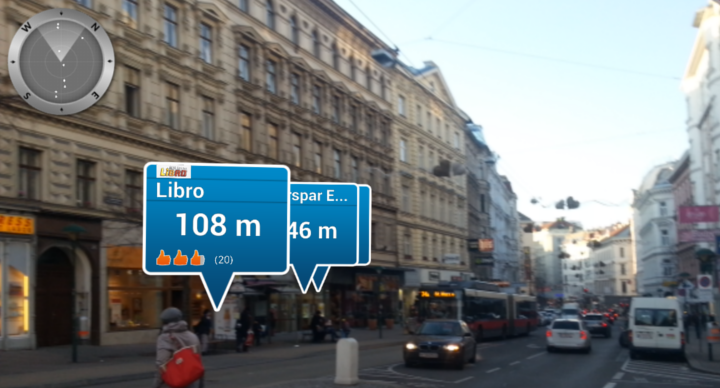
\includegraphics[width=150mm]{images/Wikitude.png}
  \caption{A Touring Machine} \label{fig:Wikitude}
\end{figure}



\section{ユーザの位置測位及びコンテキスト情報の取得に関する研究}
前節でも挙げたとおりARによるナビゲーションではユーザ位置測位やコンテキスト情報取得には様々な方式が検討されている。
前節に挙げたARナビゲーションシステムでは検討されなかった位置測位システム及びそれらを比較する研究を紹介する。


\subsection{RSSI based Bluetooth low energy indoor positioning}
RSSI based Bluetooth low energy indoor positioning\cite{7275525}


\subsection{Recent Advances in Wireless Indoor Localization Techniques and System}
Recent Advances in Wireless Indoor Localization Techniques and System\cite{Farid2013}


\section{NFCを用いて情報を取得し、ナビゲーションに応用する研究}
NFC技術を自己位置推定やコンテキスト情報取得などに利用し、ナビゲーションに役立てている研究を紹介する。

\subsection{Bridging physical and virtual worlds with electronic tags}
WantらはBridging physical and virtual worlds with electronic tags\cite{10.1145/302979.303111}で

\subsection{GoldFish}
GoldFish\cite{10.1145/2407696.2407699}は

\subsection{Development of an Indoor Navigation System Using NFC Technology}
OzdenizciらはDevelopment of an Indoor Navigation System Using NFC Technology\cite{5954491}でNFCタグを利用した室内ナビゲーションのプロトタイプ「NFC Internal」を作成している。
このプロトタイプはNFCタグにタッチすることでユーザーの現在地や向きを把握し、その情報と事前に導入した地図情報から2Dマップでの経路を提示するシステムである。(図\ref{fig:NFC_Internal})

本研究同様、施設内の各所に位置情報の書かれた近距離通信のNFCタグを設置し、タグにタッチされるたびにユーザーの場所と向きを更新している。
また屋内での位置測位に近距離通信のNFCタグを利用することの利点としてコストが少ない点、正確な位置と向きの情報が得られる点、通信の応答時間が短い点などを挙げており、これらは本研究が主張するNFCタグの採用理由の一部と一致する。
一方でユーザーへの情報提示が2Dの地図とテキストベースであることと、何度もタグにタッチすることで目的地へ最短でたどり着くことに主眼をおいている点が本研究大きく異なると言える。

\begin{figure}[h]
  \centering 
  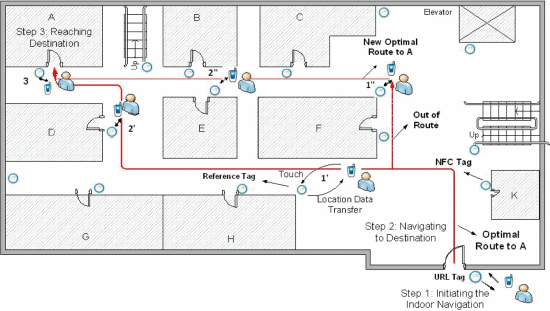
\includegraphics[width=150mm]{images/NFC_Internal.png}
  \caption{NFC Internalのイメージ} \label{fig:NFC_Internal}
\end{figure}



\section{AR・VR情報の整理・関連情報推薦にハイパーリンクを利用する研究}
ARやVRでの情報を整理するためにハイパーリンクを利用すた研究やプロジェクトを紹介する。
またハイパーリンク情報によってARとVRをシームレスに統合したシステムについても紹介する。



\subsection{VAnnotatoR}
Mehlerらが提案したVAnnotatoR\cite{10.1145/3209542.3209572}はVR/ARでのテキストや画像などのメディアをハイパーリンクを用いて管理し可視化するフレームワークである。
図\ref{fig:VAnnotatoR}のように文書や画像の他に3Dモデルや位置情報同士を関連付け、3Dでそのつながりを可視化する。
さらにユーザーの入力によって表示を変えたり関連付けられた場所ワープするような探索機能を備える。

VannotatoRはホロコーストに関連する資料を整理し、可視化することで歴史を解説するStolperwegeプロジェクトが発端となっている。そのため様々な形式の資料と位置情報を互いに関連づけた上でわかりやすく可視化・ナビゲートすることに主眼をおいている。
よってハイパーリンクを利用してARで表示する情報を管理し、それら利用して関連情報を提示するという点で本研究と設計が近いが以下の点で異なっている。
\begin{itemize} 
  \item ハイパーリンク情報の編集環境に関してwikiのような誰でも入力可能なシステムを導入していない
  \item ARの表示における位置推定は考慮に入れていない
  \item HypAR Touchでは文字情報でのみハイパーリンクを形成する
\end{itemize}

\begin{figure}[h]
  \centering 
  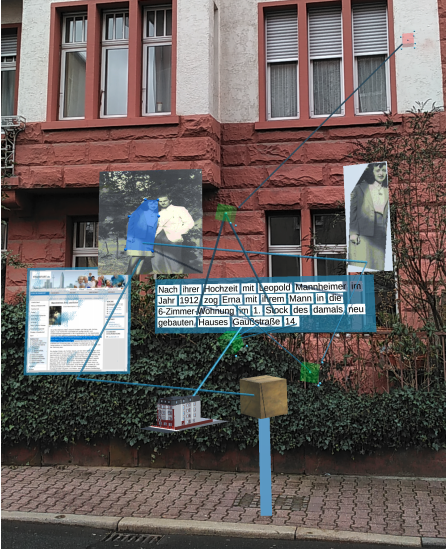
\includegraphics[width=150mm]{images/VAnnotatoR.png}
  \caption{VAnnotatoRでのAR表示} \label{fig:VAnnotatoR}
\end{figure}

\subsection{HyperReal}
RomeroらによるHyperRealは\cite{10.1145/900051.900055}

\subsection{Croquet Project}
Croquet Project\cite{10.5555/1009376.1009395}はSmithらが主導した仮想OS構築プロジェクトであり、

\subsection{Annotation authoring in collaborative 3D virtual environments}
小林らによるAnnotation authoring in collaborative 3D virtual environments\cite{10.1145/1152399.1152452}では

\subsection{MagicBook}
BillinghurstらによるMagicBook\cite{10.1145/634067.634087}は




